\chapter[Aula 4]{Espaços de Probabilidade}
\chaptermark{}





\section{Propriedades das Medidas de Probabilidade}

Um espaço de probabilidade é um tripla 
$(\Omega,\F,\P)$ onde 
\begin{itemize}
	\item 
	$\Omega$ é um conjunto chamado de espaço amostral.

	\item
	$\F$ uma $\sigma$-álgebra de subconjuntos de $\Omega$.
	Os elementos de $\F$ são chamados de eventos.
	
	\item $\P$ é uma medida de probabilidade, isto é, 
	uma função com domínio em $\F$ tomando valores em 
	$[0,1]$ satisfazendo 
		\begin{itemize}
			\item[i)] 
			$\P(E)\geq 0$ para todo $E\in \F$.

			\item[ii)] 
			$\P$ é $\sigma$-aditiva: Para qualquer
			sequência $\{E_n\}$ mutuamente disjunta 
			de eventos em $\F$ temos 
				\[
					\P\left( \bigcup_{n=1}^{\infty} E_n \right)
					=
					\sum_{n=1}^{\infty} \P(E_n).
				\]
			\item[iii)] 
			$\P(\Omega)=1$.
		\end{itemize}
\end{itemize}



Seguem das propriedade $\textrm{ii})$ e $\textrm{iii})$ acima que 
para qualquer evento $E\in\F$ vale a seguinte identidade
	\[
		P(E^c)=1-P(E).
	\]
De fato, 
	\[
		1=P(\Omega)= P(E\cup E^c)=P(E)+P(E^c).
	\]
Como toda medida de probabilidade é em particular uma medida então 
temos que 
	\[
		\P(\emptyset)=0.
	\] 
\begin{proposicao} Seja $(\Omega,\F,\P)$ um espaço de probabilidade.
Se $A,B$ são dois eventos arbitrários então 
	\[
		\P(A\cup B) = \P(A)+\P(B)-\P(A\cap B).
	\]
\end{proposicao}
\begin{proof}
Primeiro observamos que 
%	
	\begin{align*}
		\P(A) = \P(A\cap B^c)+\P(A\cap B) 
		\\
		\P(B) = \P(B\cap A^c)+\P(B\cap A) 
	\end{align*}
Note que podemos escrever $A\cup B = (A\cap B^c) \cup (B\cap A^c) \cup (A\cap B)$.
Tomando probabilidade em ambos lados desta igualdade 
e usando as identidades acima, temos
	\begin{align*}
	\P(A\cup B) 
	&=
	\P(A\cap B^c) + \P(B\cap A^c) + \P(A\cap B)
	\\
	&=
	[\P(A)-\P(A\cap B)] + [\P(B)-\P(A\cap B)] + P(A\cap B)
	\\
	&=
	\P(A)+\P(B)-\P(A\cap B).
	\end{align*}


\end{proof}

\begin{teorema}[Fórmula de Inclusão-Exclusão]
Para quaisquer eventos $E_1,\ldots,E_n$ temos 
	\begin{align*}
		\P\left( \bigcup_{j=1}^{n} E_j \right)
		&=
		\sum_{j=1}^n \P(E_j)
		-
		\sum_{1\leq i<j\leq n} \P(E_i\cap E_j) 
		+
		\sum_{1\leq i<j<k\leq n} \P(E_i\cap E_j\cap E_k)-\ldots
		\\[0.3cm]
		&\hspace*{0.5cm} \ldots(-1)^{n+1} \P(E_1\cap\ldots\cap E_n).
	\end{align*}
\end{teorema}

\begin{proof}
 Podemos provar o teorema por indução. Para $n=2$ o teorema
 segue diretamente da proposição acima. Para dar o passo de 
 indução basta escrever $\cup_{j=1}^{k+1} E_j$ 
 como $\cup_{j=1}^{k}E_j\cup E_{k+1}$, usar o caso $n=2$ 
 para calcular a probabilidade desta decomposição, em seguida usar 
 a hipótese de indução para 
 \[	
 \P \left( \bigcup_{j=1}^{k} E_j \right)
 \qquad
 \text{e}
 \qquad
 \P \left( \bigcup_{j=1}^{k} (E_j\cap E_{k+1}) \right)
 \]
 e reorganizar os termos de ambas as somas. Observe 
 por exemplo, que as probabilidades de interseções de pares 
 com $E_j$'s com índice menores ou iguais a $k$ virão 
 da primeira probabilidade e interseção de pares de
 eventos $E_j$'s onde um dos eventos é $E_{k+1}$ virá 
 da segunda soma e assim por diante.
\end{proof}

Uma aplicação deste Teorema é a obtenção das
chamadas {\bf Desigualdades de Bonferroni} \index{Desigualdade!Bonferroni}.
A prova destas desigualdades segue simplesmente de negligenciarmos 
os resto. Dois exemplos de tais desigualdades são mostrados
abaixo:
\[ 
\begin{array}{c}
	\displaystyle
	\P \left( \bigcup_{j=1}^{n} E_j \right) 
	\leq 
	\sum_{j=1}^n \P(E_j)
	%
	%
	\\[0.5cm]
	%
	%
	\displaystyle
	\P \left( \bigcup_{j=1}^{n} E_j \right) 
	\geq
	\sum_{j=1}^n \P(E_j) - \sum_{1\leq i<j\leq n} \P(E_i\cap E_j)	
\end{array}
\]

Outra propriedade importante é a {\bf Monotonicidade} de $\P$, isto é, 
para quaisquer eventos $A,B$ tais que $A\subset B$ temos 
$\P(A)\leq \P(B)$. De fato, 
$\P(B)=\P(B\cap A)+\P(B\cap A^c)= \P(A)+\P(B\setminus A)\geq \P(A)$.

Toda medida de probabilidade é $\sigma$-subaditiva, ou seja, 
para quaisquer eventos $E_1,E_2,\ldots$ temos 
	\[
		\P\left( \bigcup_{n=1}^{\infty} E_n\right)
		\leq 
		\sum_{n=1}^{\infty} \P(E_n).
	\]
Para verificar que esta propriedade é verdadeira basta observar que 
\[
	\bigcup_{n=1}^{\infty} E_n = E_1 \cup (E_1^c\cap E_2) \cup (E_1^c\cap E_2^c\cap E_3) \cup \ldots
\]
aplicar a $\sigma$-aditividade de $\P$ e em seguida usar a monotonia
obtendo
	\begin{align*}
	\P\left( \bigcup_{n=1}^{\infty} E_n\right)
	&=
	\P(E_1)+\P(E_1^c\cap E_2) + \P(E_1^c\cap E_2^c\cap E_3) +\ldots
	\\
	&\leq
	\P(E_1) + \P(E_2) + \P(E_3) +\ldots
	\end{align*}
	
\begin{teorema}[Continuidade da Probabilidade]
	Sejam $(\Omega,\F,\P)$ um espaço de Probabilidade e
	$\{E_n\}$ uma sequência de eventos neste espaço.
	\begin{enumerate}
		\item
		Se $E_n\nearrow E$ então 
		$\displaystyle\lim_{n\to\infty}\P(E_n)=\P(E)$.
		\item 
		Se $E_n\searrow E$ então 
		$\displaystyle\lim_{n\to\infty}\P(E_n)=\P(E)$.		
	\end{enumerate}
\end{teorema}

\begin{proof}
Vamos provar o primeiro item do Teorema. 
Suponha que $E_1\subset E_2\subset \ldots\subset E_n\subset \ldots$
e defina a seguinte sequência de eventos 
\[
B_1= E_1,\ B_2= E_2\setminus E_1,\ \ldots,\  B_n=E_n\setminus E_{n-1}.
\]
Por construção a sequência $\{B_n\}$ é uma sequência de eventos
mutuamente disjunta e além do mais 
\[
\bigcup_{j=1}^n B_j = E_n, \quad 
\bigcup_{j=1}^{\infty} B_j = \bigcup_{j=1}^{\infty} E_j = E.
\]
Da $\sigma$-aditividade segue que 
\begin{align*}
	\P(E)
	&=
		\P\left( \bigcup_{n=1}^{\infty} E_n\right)
		=
		\sum_{n=1}^{\infty}\P(B_n)
		=
		\lim_{n\to\infty} \sum_{j=1}^n \P(B_j)
	\\[0.3cm]
	&=
		\lim_{n\to\infty}\P\left( \bigcup_{j=1}^{n} B_j\right)
		=
		\lim_{n\to\infty}\P\left( E_n\right).
\end{align*}

Para provar o segundo item note que se $E_n\searrow E$ 
então $E_n^c \nearrow E^c$. Aplicando o resultado que 
acabamos de provar temos que 
	\[
		1-\P(E)
		=
		\P(E^c)		
		=
		\lim_{n\to\infty} \P(E_n^c)
		=
		\lim_{n\to\infty} [1-\P(E_n)]		
	\]
de onde segue o resultado.
\end{proof}

Vamos provar agora um lema de continuidade para sequências 
que não são necessariamente monótonas. 
Este lema será chamado de lema de Fatou para funções indicadoras
e a razão para isto ficará clara futuramente.

\begin{lema}[Lema de Fatou para Funções Indicadoras]
\label{lema-fatou-indicadoras}
Seja $(\Omega,\F,\P)$ um espaço de probabilidade e 
$\{E_n\}$ uma sequência de eventos.
\begin{enumerate}
	\item
	$\displaystyle
	\P(\liminf_{n\to\infty} E_n)
	\leq 
	\liminf_{n\to\infty} \P(E_n)
	\leq
	\limsup_{n\to\infty} \P(E_n)
	\leq
	\P(\limsup_{n\to\infty} E_n)$.
	
	\item Se $E_n\to E$ então $\P(E_n)\to \P(E)$.
\end{enumerate}
\end{lema}


\begin{proof}
Primeiro vamos assumir que 1 é válido e vamos mostrar 2.
Suponha que $E_n\to E$. Então 
\[
 \liminf_{n\to\infty} E_n = \limsup_{n\to\infty} E_n = E.
\]
Aplicando 1 temos que 
	\begin{align*}
	\P(E)
	&=\displaystyle
		\P(\liminf_{n\to\infty} E_n)
		\leq 
		\liminf_{n\to\infty} \P( E_n)
		\leq
		\limsup_{n\to\infty}\P(E_n)
		\leq
		\P(\limsup_{n\to\infty} E_n)
		=
		P(E).
	\end{align*}
O que prova que $\P(E_n)\to P(E)$.

Passamos agora a prova do item 1. Por definição 
do $\liminf$, continuidade da probabilidade
temos 
\begin{align*}
	\P(\liminf_{n\to\infty} E_n)
	&=
	\P\left( \lim_{n\to\infty} \bigcap_{k\geq n}E_k \right)
	\\
	&=
	\lim_{n\to\infty} \P\left( \bigcap_{k\geq n}E_k \right)
\end{align*}
Por monotonicidade temos que 
	\[
		\P\left( \bigcap_{k\geq n}E_k \right)
		\leq 
		\P(E_n).
	\] 
Assim se tomamos $\liminf$ em ambos os lados e usamos as igualdades acima,
obtemos a seguinte desigualdade
	\begin{align*}
	\P(\liminf_{n\to\infty} E_n)
	\leq 
	\liminf_{n\to\infty}\P(E_n).
\end{align*} 

De maneira análoga, temos 
\begin{align*}
	\P(\limsup_{n\to\infty} E_n)
	&=
	\P\left( \lim_{n\to\infty} \bigcup_{k\geq n}E_k \right)
	\\[0.2cm]
	&=
	\lim_{n\to\infty} \P\left( \bigcup_{k\geq n}E_k \right)
	\\[0.3cm]
	&\geq 
	\limsup_{n\to\infty} \P(E_n).
\end{align*}
\end{proof}



\section{Função Distribuição}

\begin{exemplo}
Seja $\Omega=\R$ (conjunto dos números reais) e $\P$ uma medida de probabilidade em $\R$.
Defina $F:\mathbb{R}\to [0,1]$ por 
	\[
		F(x) =\P((-\infty,x]).
	\]
Então 
\begin{enumerate}
	\item	
	$F$ é contínua a direita.
	
	\item
	$F$ é monótona não-decrescente	
		
	\item 
	Existem os seguintes limites 
		\begin{itemize}
			\item 
 			$\displaystyle\lim_{x\to+\infty} F(x)=1$		
			
			\item
			$\displaystyle\lim_{x\to -\infty} F(x)=0$.
		\end{itemize}
\end{enumerate}
\end{exemplo}
\begin{proof}
	Vamos mostrar primeiro o item 2. Se $x<y$ então temos que 
	$(-\infty,x]\subset (-\infty,y]$. O resultado segue diretamente 
	da monotonicidade de $\P$ e da definição de $F$.
	
	Passamos agora para a prova do item 3.  Considere uma subsequência
	 $\{x_{n_j}\}\subset \{x_n\}$ monótona 	crescente  com
	  $x_{n_{j}}\to \infty$,  como $(-\infty, x_{n_j}]$ é uma sequência 
	  encaixada crescendo  para $\mathbb{R}$, segue da continuidade da probabilidade 
	  que    
	  \[
	  \lim_{n\to \infty} F(x_{n_j})=1
	  \]
ou seja  dado  $\epsilon>0$ existe $n_{j_0}$ tal que para todo $n_j>n_{j_0}$ 
vale que $F(x_{n_j})>1-\epsilon$. Como $x_n\to \infty$ temos que 
existe $N$ tal que para todo $n>N$ tem-se $x_n> x_{n_{j_0}}$
 portanto da monotonicidade de $F$ segue que $F(x_n)>1-\epsilon$
  para todo $n>N$ donde segue o item 3.	
	 O cálculo do outro limite 
do item 3 é análoga, bastando agora usar a continuidade no 
vazio. 

Para provar o item 1 temos que mostrar que sempre que 
$x_n \downarrow x$ temos que $F(x_n) \downarrow F(x)$.
Mas isto é consequência imediata da propriedade de continuidade
de $\P$ e de que 
	\[
		(-\infty,x_n] \searrow (-\infty,x].
	\]
\end{proof}







\begin{definicao}[Função Distribuição]
Uma função $F:\mathbb{R}\to [0,1]$ satisfazendo 
as seguintes propriedades:
\begin{enumerate}
	\item	
	$F$ é contínua a direita.
	
	\item
	$F$ é monótona não-decrescente	
		
	\item 
	Existem os seguintes limites 
		\begin{itemize}
			\item 
 			$\displaystyle\lim_{x\to+\infty} F(x)=1$		
			
			\item
			$\displaystyle\lim_{x\to -\infty} F(x)=0$.
		\end{itemize}
\end{enumerate}
é chamada de uma função distribuição.
\end{definicao}






\section{Construção de $\P_{F}$}

O objetivo nesta seção é construir uma 
medida de probabilidade em $\R$ com uma 
dada função distribuição $F$. 
Em outras palavras, vamos construir
uma medida $\P_F$ tal que 
\[
	\P_{F}((-\infty,x]) = F(x).
\]
Para construir tal probabilidade
vamos precisar da medida de Lebesgue que 
nesta seção será denotada por $\lambda$.


Vamos começar definindo uma função contínua a 
esquerda $G:(0,1)\to\R$ que é uma espécie de 
``inversa generalizada'' de $F$.
Esta função é definida da seguinte maneira:
para cada $y\in (0,1)$ definimos 
	\[
		G(y)
		\equiv 
		\inf\{ s\in\R: y\leq F(s)\} 
		= 
		\inf \{ F^{-1}([y,+\infty))\}.
	\]
Para simplificar a notação vamos escrever
	\[
	 	A(y)\equiv \{ s\in\R: y\leq F(s)\}
	\]	

\begin{exercicio}
 Mostre que a função $G$ dada acima está bem definida,
 isto é, para todo $y\in (0,1)$ temos que 
 $A(y)\neq \emptyset$ e que seu ínfimo pertence a $\R$.
\end{exercicio}

\begin{observacao}
Em geral, $G$ {\bf não} é uma função injetiva. 
Por exemplo, se 
$x_0$ é um ponto de descontinuidade de $F$ então 
para qualquer ponto $y$ pertencente ao 
intervalo aberto $I_0=(F(x_0-),F(x_0))$ temos  
$G(y)=x_0$, veja figura abaixo:
%%%  Figura sobre Inversa Generalizada
\begin{center}
\begin{figure}[!htb]
\centering
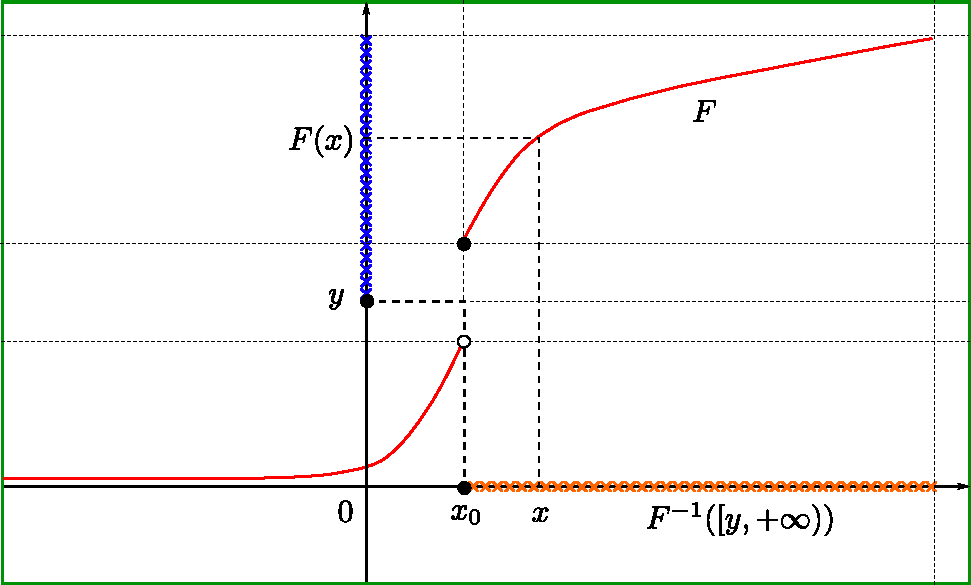
\includegraphics[width=0.8\textwidth]{Figuras/inversa-gen.pdf}
\caption{Esboço do gráfico de uma função distribuição $F$ descontínua.}
\label{Rotulo}
\end{figure}
\end{center}
%%%
\end{observacao}

\begin{proposicao}\label{prop-propriedades-G}
	Para todo $y\in (0,1)$ o conjunto $A(y)$ definido acima 
	tem as seguintes propriedades:
	\begin{enumerate}
		\item 
		$A(y)$ é um conjunto fechado.
		
		\item
		$\inf A(y) \in A(y)$, ou seja, $y\leq F(G(y))$.
		
		\item 
		$t<G(y)$ se, e somente se, $F(t)<y$.
		
		\item 
		$G(y)\leq t$ se, e somente se, $y\leq F(t)$.
	\end{enumerate}
\end{proposicao}


\begin{proof}
	{\bf Prova do item 1.} 
	Seja $\{s_n\}$ uma sequência em $A(y)$ tal que $s_n\to s$. 
	Note que $\{s_n\}$ possui pelo menos uma subsequência 
	monótona, não-crescente ou não-decrescente $\{s_{n_{k}}\}$ 
	que converge para $s$. Vamos considerar primeiro o caso 
	em que existe uma subsequência $s_{n_k}\downarrow s$. 
	Já que $s_{n_k}\in A(y)$ então 
	é válida a seguinte desigualdade $y\leq F(s_{n_k})$.
	Tomando nesta desigualdade o limite, quando $k\to\infty$, 
	obtemos da continuidade a direita de $F$ que 
		\[ 
			y \leq 
			\lim_{k\to\infty} F(s_{n_k}) 
			= 
			F(s).
		\]
	O que mostra que $s\in A(y)$.
	Por outro lado, se $\{s_n\}$ não possui uma subsequência 
	$s_{n_k}\downarrow s$, então existe no máximo uma quantidade
	finita de pontos da sequência $\{s_n\}$ 
	que é maior ou igual a $s$.
	Assim podemos afirmar que existe pelo menos 
	uma subsequência $s_{n_k}\uparrow s$
	tal que $s_{n_k} < s$. Usando  
	a definição de $A(y)$ e a monotonicidade de $F$ 
	temos que 
		\[
			y\leq F(s_{n_k})\leq F(s).
		\]
	Logo $s\in A(y)$ e isto conclui a prova de que $A(y)$ é 
	um subconjunto fechado da reta.
	
	{\bf Prova do item 2.} Segue diretamente da definição $\inf A(y)$,
	que 	existe uma sequência $\{s_n\}\subset A(y)$ tal que $s_n\to \inf A(y)$.
	Uma vez que o item 1 garante que $A(y)$ é fechado, temos que 
		\[G(y)=\inf A(y) \in A(y).\]
	 Segue então da definição de $A(y)$ que $y\leq F(G(y))$.


	{\bf Prova do item 3.} Note que $t<G(y)$ é equivalente a
	$t<\inf A(y)$. Esta desigualdade é equivalente a 
	$t\in A(y)^c$, isto é, $t\in\{s\in\R: F(s)<y\}$. 
	Como a última afirmação é equivalente a $F(t)<y$ a
	prova deste item está completa.
	
	
	{\bf Prova do item 4.} Se $G(y)\leq t$ então 
	segue do item 3 que 	$y\leq F(t)$. A recíproca é 
	também uma aplicação direta do item 3.  
	Isto completa a prova da proposição.
\end{proof}

\bigskip

Para cada $A\subset \R$ definimos agora o seguinte conjunto:
	\begin{equation}\label{def-xi-F}
		\xi_F(A) \equiv \{ x\in (0,1]: G(x)\in A \} = G^{-1}(A)\cap (0,1].
	\end{equation}
No lema seguinte mostramos que se $A$ 
é um boreliano de $\R$ (notação $A\in\mathscr{B}(\R)$)  
então 
$\xi_F(A)$ é um boreliano de $(0,1]$ 
(notação $\xi_F(A) \in\mathscr{B}((0,1])$).

\begin{lema}
	Se $A\in\mathscr{B}(\R)$ então $\xi_F(A) \in\mathscr{B}((0,1])$, onde
	$\xi_F(A)$ é definido como em \eqref{def-xi-F}.
\end{lema}



\begin{proof}
Considere a seguinte coleção 
	\[
		\mathscr{C} 
		=
		\{ A\subset\R: \xi_F(A) \in \mathscr{B}((0,1])\}.
	\]
Afirmamos que $\mathscr{C}$ contém qualquer intervalo finito da forma
$(a,b]\subset \R$. De fato, segue dos itens 3 e 4 
da Proposição \ref{prop-propriedades-G} que 
para todo $x\in (0,1)$ satisfazendo 
$a<G(x)$ temos $F(a)<x$ e por outro lado, se $G(x)\leq b$ temos 
$x\leq F(b)$. Da definição de $\xi_{F}(A)$ e 
das duas observações anteriores temos que
%
%
\begin{align*}
	\xi_F((a,b]) 
	&= 
	\{ x\in (0,1]: G(x) \in (a,b] \}
	\\
	&=	
	\{ x\in (0,1]: a<G(x)\leq b  \}
	\\
	&=
	\{ x\in (0,1]:F(a) <x \leq F(b) \}
	\\
	&=
	(F(a),F(b)].
\end{align*}
Como o lado direito acima pertence a $\mathscr{B}((0,1])$
segue que todo intervalo finito $(a,b]\in \mathscr{C}$.
Em outras palavras, a coleção $\mathscr{C}$ 
contém o $\pi$-sistema $\mathcal{G}=\{ (a,b]: a,b\in\R\}$.


Vamos mostrar agora que $\mathscr{C}$ é um $\lambda$-sistema. 
Para provar que $\R\in \mathscr{C}$, basta 
notar que
$
	\xi_F(\R)
	= G^{-1}(\mathbb{R})\cap (0,1] 
	= (0,1)\cap (0,1]
	\in \mathscr{B}((0,1]). 
$
Suponha que $A\in\mathscr{C}$, então 
$\xi_F(A)=G^{-1}(A)\cap (0,1]\in \mathscr{B}((0,1])$.
Pela propriedades de imagem inversa temos que 
\[
	G^{-1}(A^c)= \Big(G^{-1}(A)\Big)^c
\]
e como $\xi_F(A)$ é um boreliano de $(0,1]$, segue da definição 
de topologia induzida que 
	\[
		\xi_F(A^c)
		=
		G^{-1}(A^c)\cap (0,1]
		= 
		\Big(G^{-1}(A)\Big)^c\cap (0,1]		
	\]
é um boreliano de $(0,1]$, mostrando que $A^c\in\mathscr{C}$.

Se $\{A_n\}$ é uma família de 
conjuntos mutuamente disjuntos em $\mathscr{C}$,
então 
	\begin{align*}
	\xi_F\left( \bigcup_{n=1}^{\infty} A_n\right)
	=&
	G^{-1}\left( \bigcup_{n=1}^{\infty} A_n\right)\cap (0,1]
	\\
	=&
	\bigcup_{n=1}^{\infty} G^{-1}\left(A_n \right)\cap (0,1]
	\end{align*}
pertence a $\mathscr{B}((0,1])$. Logo $\cup_{n\geq 1} A_n\in \mathscr{C}$
o que prova encerra a prova de que $\mathscr{C}$ é um $\lambda$-sistema.

Pelo Teorema $\pi-\lambda$ de Dynkin $\mathscr{C}$ contém a $\sigma$-álgebra
gerada por $\mathcal{G}$ que é $\mathscr{B}(\R)$. Este fato 
completa a prova do lema.
\end{proof}

Finalmente podemos apresentar a definição de $\P_F$.
Para cada $A\in \mathscr{B}(\R)$ definimos 
	\[
		\P_{F}(A) =\lambda(\xi_{F}(A)),
	\]
onde $\lambda$ é a medida de Lebesgue em $(0,1]$.
É simples verificar que $\P_F$ é de fato uma medida
de probabilidade sobre $\mathbb{R}$ 
e que a função distribuição que ela induz é dada por
%
\begin{align*}
	\P_F((-\infty,x]) 
	&=
	\lambda \Big(\xi_{F}((-\infty,x])\Big)
	\\
	&=
	\lambda\Big( \{ y\in (0,1]: G(y)\in (-\infty,x] \} \Big)
	\\
	&=
	\lambda\Big( \{ y\in (0,1]: G(y)\leq x \} \Big)
	\\
	&=
	\lambda\Big( \{ y\in (0,1]: y\leq F(x) \} \Big)
	\qquad
	(\text{item 4 Proposição \ref{prop-propriedades-G}})
	\\
	&=
	\lambda\Big( (0,F(x)] \Big)
	\\
	&=
	F(x).
\end{align*}














